\chapter{Question 3}
\label{available-representation}

\textbf{Estimate the age of each of the 1000 URIs using the "Carbon Date" tool: }
\url{http://ws-dl.blogspot.com/2014/11/2014-11-14-carbon-dating-web-version-20.html}\\

\textbf{Note: you'll should download the library and run it locally; don't try to use the web service.
For URIs that have $>$ 0 Mementos and an estimated creation date, create a graph with age (in days) on one axis and number of mementos
on the other.  
Not all URIs will have Mementos, and not all URIs will have an estimated creation date.  State how many fall into either categories. }

\begin{itemize}
\item I downloaded the `Carbon Date' tool from {\url{http://ws-dl.blogspot.com/2014/11/2014-11-14-carbon-dating-web-version-20.html}}. 
\item With the help of this tool, estimated creation date of URIs is obtained.
\item I carbon dated URIs which had mementos $>$ 0. This is outlined in Listing \ref{lst:code1}.
\item Furthermore I parsed the estimated creation date if any and calculated the age of each URI in days using `getCreatedTime.py'.. This is outlined in Listing \ref{lst:code2}.
\item Figure \ref{fig:fig1} illustrates a graph with Mementos on x-axis and Age(in days) on y-axis. Looking at the graph I observe that for most of the URIs, as the number of mementos increases age also increases.
\item Figure \ref{fig:fig2} illustrates the data of Age(in Days) and Number of mementos, with Number of mementos in ascending order. 
\item If I run the code for all the 1000 URIs, 525 URIs did not have estimated Creation date. But if I consider only the URIs that have $>$ 0 mementos then all of them have an Estimated creation date.
\item Out of the  1000 URIs, 151 URIs fulfilled the given criteria of having $>$ 0 Mementos and an estimated creation date. 
\end{itemize}

\newpage
\begin{figure}[h!]
\begin{center}
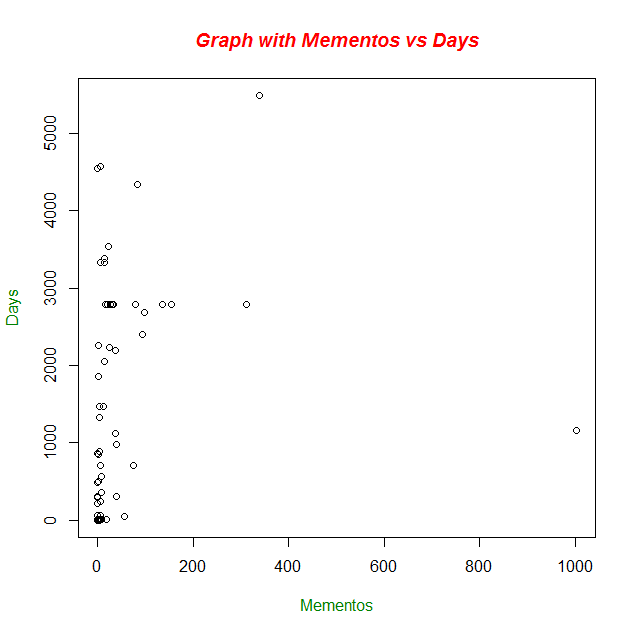
\includegraphics[scale=0.55, keepaspectratio=true]{figures/q3graph.png}
\caption{Graph for Mementos vs age}
\label{fig:fig1}
\end{center}
\end{figure}

\newpage
\begin{figure}[h!]
\begin{center}
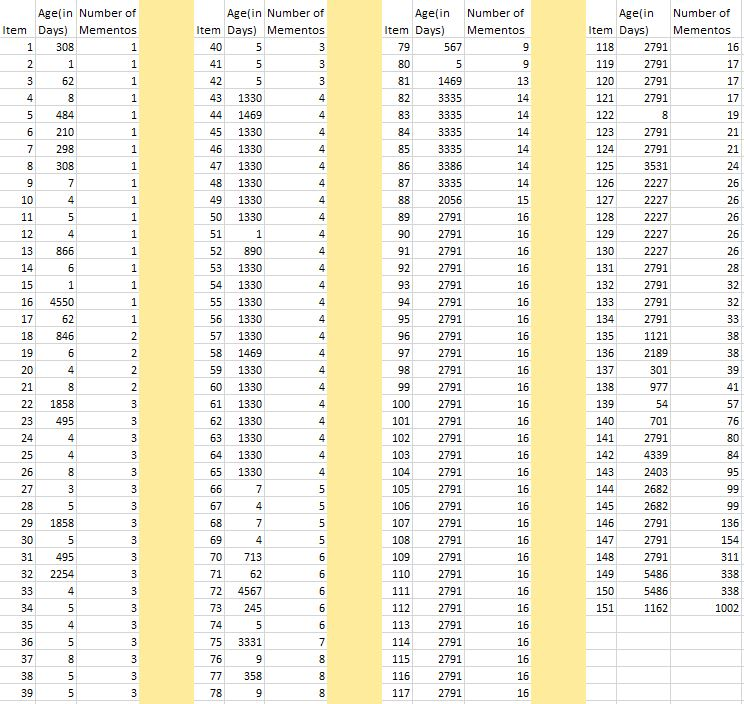
\includegraphics[scale=0.55, keepaspectratio=true]{figures/data.JPG}
\caption{Data for Number of Mementos and age}
\label{fig:fig2}
\end{center}
\end{figure}

\newpage
\textbf{Code Listing}
\lstinputlisting[language=Python,caption=``Python code which takes URIs $>$ 0 Mementos as input and writes the JSON output with Estimated Creation date into a file.'',frame=single,label=lst:code1,breaklines=true,captionpos=b,numbers=left,showspaces=false,showstringspaces=false,basicstyle=\footnotesize]{src/local.py}

\newpage
\textbf{Code Listing}
\lstinputlisting[language=Python,caption=``Python code for calculating age of URI in days and writing them into a file'',frame=single,breaklines=true,label=lst:code2,captionpos=b,numbers=left,showspaces=false,showstringspaces=false,basicstyle=\footnotesize]{src/getCreatedTime.py}




